\documentclass[a4paper]{article}

% --- Packages ---

\usepackage{a4wide}
\usepackage[utf8]{inputenc}
\usepackage{amsmath}
\usepackage{mathtools}
\usepackage{amssymb}
\usepackage[english]{babel}
\usepackage{mdframed}
\usepackage{systeme,}
\usepackage{lipsum}
\usepackage{relsize}
\usepackage{caption}
\usepackage{tikz}
\usepackage{tikz-3dplot}
\usetikzlibrary{shapes.geometric}
\usepackage{pgfplots}
\usepackage{pgfplotstable}
\pgfplotsset{compat=newest}%1.7}
\usepackage{harpoon}%
\usepackage{graphicx}
\usepackage{wrapfig}
\usepackage{subcaption}
\usepackage{authblk}
\usepackage{float}
\usepackage{listings}
\usepackage{xcolor}
\usepackage{chngcntr}
\usepackage{amsthm}
\usepackage{comment}
\usepackage{commath}
\usepackage{hyperref}%Might remove, adds link to each reference
\usepackage{url}
\usepackage{calligra}

% --- Bibtex ---

%\usepackage[backend = biblar,]{bibtex}

%\addbibliografy(ref.bib)

% --- Commands --- 

\newcommand{\w}{\omega}
\newcommand{\trace}{\text{Tr}}
\newcommand{\grad}{\mathbf{\nabla}}
%\newcommand{\crr}{\mathfrak{r}}
\newcommand{\laplace}{\nabla^2}
\newcommand{\newparagraph}{\vspace{.5cm}\noindent}

% --- Math character commands ---

\newcommand{\curl}[1]{\mathbf{\nabla}\times \mathbf{#1}}
\newcommand{\dive}[1]{\mathbf{\nabla}\cdot \mathbf{#1}}
\newcommand{\res}[2]{\text{Res}(#1,#2)}
\newcommand{\fpartial}[2]{\frac{\partial #1}{\partial #2}}
\newcommand{\rot}[3]{\begin{vmatrix}\hat{x}&\hat{y}&\hat{z}\\\partial_x&\partial_y&\partial_z\\#1&#2&#3 \end{vmatrix}}
\newcommand{\average}[1]{\langle #1 \rangle}
\newcommand{\ket}[1]{|#1\rangle}
\newcommand{\bra}[1]{\langle #1|}


%  --- Special character commands ---

\DeclareMathAlphabet{\mathcalligra}{T1}{calligra}{m}{n}
\DeclareFontShape{T1}{calligra}{m}{n}{<->s*[2.2]callig15}{}
\newcommand{\crr}{\mathcalligra{r}\,}
\newcommand{\boldscriptr}{\pmb{\mathcalligra{r}}\,}


\title{FK8028: Report 2}
\author{Author : Andreas Evensen}
\date{Date: \today}

% --- Code ---

\definecolor{codegreen}{rgb}{0,0.6,0}
\definecolor{codegray}{rgb}{0.5,0.5,0.5}
\definecolor{codepurple}{rgb}{0.58,0,0.82}
\definecolor{backcolour}{rgb}{0.95,0.95,0.92}

\lstdefinestyle{mystyle}{
    backgroundcolor=\color{backcolour},   
    commentstyle=\color{codegreen},
    keywordstyle=\color{magenta},
    numberstyle=\tiny\color{codegray},
    stringstyle=\color{codepurple},
    basicstyle=\ttfamily\footnotesize,
    breakatwhitespace=false,         
    breaklines=true,                 
    captionpos=b,                    
    keepspaces=true,                 
    numbers=left,                    
    numbersep=5pt,                  
    showspaces=false,                
    showstringspaces=false,
    showtabs=false,                  
    tabsize=2
}

\lstset{style=mystyle}

\begin{document}

\thispagestyle{empty}
\begin{titlepage}
   \begin{center}
       % \vspace*{1cm}
       \huge
       \textbf{Molecular dynamics: Argon Fluid}\\
       \vspace*{1cm}
       \textbf{Course: FK8028}
       \large

       \vspace*{0.5cm}
       \textbf{Author: Andreas Evensen}\\
       \vspace*{.5cm}
       \small
       \vspace*{1.cm}
       \textbf{Submission date: \today}\\
       \vspace*{.5cm}
       \vspace{0.8cm}
     
       \small
       Stockholm University\\
       Computational Physics\\
       Sweden\\
   \end{center}
\end{titlepage}
\pagenumbering{Roman}
\newpage
\pagenumbering{roman}
\setcounter{page}{1}
\newpage
\tableofcontents
\newpage
\pagenumbering{arabic}
\section{Introduction}
In this report one investigates how multiple Argon atoms interact when in gas-phase. The atoms' interaction is modeled by the Lennard-Jones potential.
One implemented a time-integration method, the Velocity Verlet method, to simulate the atoms' motion.
Furthermore, Periodic Boundary Conditions (PBC) was implemented, with position wrapping, to simulate an infinite gas.

\newparagraph
One found that the symplectic behavior of the Velocity Verlet method, which conserves the Hamiltonian, was conserved in the simulations, after velocity rescaling had ceased. Moreover, one also found that the temperature of the system fluctuates.
\section{Theory and Method}
Interactions between two atoms, with relative position $\mathbf{r}$ can be expressed as a potential energy $\mathcal{V}(\mathbf{r})$; in this report one focuses on the Lennard-Jones potential, which is given by the following equation \eqref{eq: Lennard-Jones potential}:
\begin{align}
    \mathcal{V}(\mathbf{r}) &= \epsilon\left[\left(\frac{\sigma}{\abs{\mathbf{r}}}\right)^{12} + \left(\frac{\sigma}{\abs{\mathbf{r}}}\right)^6\right].\label{eq: Lennard-Jones potential}
\end{align}The force, $\mathbf{F} = -\grad \mathcal{V}$, then allows to find the acceleration, $\mathbf{a} = \mathbf{F}/m$, where $m$ is the mass of the atom. In this, case, one assumes that the one has a uniform gas, and thus all the atoms has the same mass, $m = 39.948$~amu[1].
With this one can find the position of the atoms as a function of time, $x(t)$, and the velocity as a function of time, $v(t)$ via the Velocity Verlet method:
\begin{align*}
    \mathbf{r}(t + \Delta t) &= \mathbf{r}(t) + \mathbf{v}(t)\Delta t + \frac{1}{2}\mathbf{a}(t)\Delta t^2,\\
    \mathbf{v}(t + \Delta t) &= \mathbf{v}(t) + \frac{1}{2}\left[\mathbf{a}(t) + \mathbf{a}(t + \Delta t)\right]\Delta t.
\end{align*}From this one can find the kinetic energy, $\mathcal{K} = \sum_i \frac{1}{2}m\dot{\mathbf{r}}_i(t)^2$, and the potential energy, $\mathcal{V}(\mathbf{r})$ of the system. The Hamiltonian of the system is then given by:
\begin{align*}
    \mathcal{H} &= \mathcal{K} + \mathcal{V}.
\end{align*}

\newparagraph
In this report, everything is presented in terms of units in electron-volts (eV), Ångström (Å) and seconds (s), thus $\mathbf{r}$~$[$Å$]$, $\mathbf{v}$~$[$Å$/$s$]$, $\mathbf{a}$~$[$Å$/$s$^2]$, $\mathcal{V}$~$[$eV$]$, $\mathcal{K}$~$[$eV$]$, $\mathcal{H}$~$[$eV$]$, and $m$~$[$eVs$^2/$Å$^2]$.


\subsection{Bouncing test}\label{sec: Bouncing test method}
When two atoms are placed close to their equilibrium position, $r_{eq} \approx 3.8$~Å for argon atoms, they start to oscillate. This is a result of the atoms being trapped in an energy well and thus oscillate back and forth. 
This is often referred to as the bouncing test, and is a decent way to test the implementation of the Velocity Verlet method. In this report, one implements Periodic Boundary Conditions, and position wrapping. To ensure that the method is implemented correctly, one checks this via the bouncing test.

\newparagraph
The atoms are placed at a distance $6$~Å apart in the $\hat{x}$ direction, and are given an initial velocity of $0$~Å$/$s. The box-length is set to be $10$~Å. The atoms then have a stronger interaction with the closest atom in the other image, which means that the atoms will bounce back and forth between the two images. This is a good way to test the implementation of the PBC and position wrapping.

\subsection{Gas}
The volume of a gas can be expressed as the following:
\begin{align*}
    V = \frac{m}{\rho},
\end{align*}where, if one assumes a cubic volume, the length can be expressed as $L = (m/\rho)^{1/3}$. Periodic Boundary Conditions are enforced by the minimum image convention.
The minimum image convention is a method to enforce the periodic boundary condition and is done by finding the closest image of the atom in the neighboring box. This is done by the following:
\begin{align*}
    \mathbf{r}= \mathbf{r} - L\cdot\text{round}\left(\frac{\mathbf{r}}{L}\right),
\end{align*}where $L$ is then the box-length and $\mathbf{r}$ is the position vector. To implement the PBC one utilizes so-called position wrapping, which is done by the following:
\begin{align*}
    \mathbf{r} = \mathbf{r} - L\cdot\left\lfloor\frac{\mathbf{r}}{L}\right\rfloor,
\end{align*}where again $L$ is the box-length and $\mathbf{r}$ is the position vector. The floor function determines whether the position exceeds the box-length, and if so, wraps the position back to the other side of the box. This is done for all three dimensions. The force between the atoms is given by the Lennard-Jones potential \eqref{eq: Lennard-Jones potential}.

\newparagraph
Velocity rescaling is a method to ensure that the temperature of the system is constant. This is done by rescaling the velocity of the atoms, which is done by the following:
\begin{align}
    T &= \frac{2}{3Nk_B}\sum_i \frac{1}{2}m\abs{\mathbf{v}_i}^2,\nonumber\\
    T' &= \frac{2}{3Nk_B}\sum_i \frac{1}{2}m\abs{a\mathbf{v}_i}^2,\nonumber\\
    \implies a &= \sqrt{\frac{T'}{T}}.\label{eq: velocity rescaling}
\end{align}Thus, if the temperature of the system is at a temperature $T$ and one wants to change it to a temperature $T'$, one rescales the velocity by a factor $a$. This however, changes the kinetic energy of the system, and thus the Hamiltonian, $\mathcal{H}(t) = \mathcal{K}(t) + \mathcal{V}(t)$, is no longer conserved.
To minimize the introduced error, one only rescales the velocity in the beginning of the simulation. 

\section{Result and Discussion}
This section is dedicated to presenting the results of the simulations, as well as discussing them. This section is divided into two parts: the bouncing test, sec \ref{sec: Bouncing test} and the gas, sec \ref{sec: Gas}.

\subsection{Bouncing test}\label{sec: Bouncing test}
With the initial conditions discussed in sec \ref{sec: Bouncing test method}, one finds that the atoms oscillate back and forth between the two images. This is visible in \ref{fig: Position BT}, where the position of the atoms is plotted as a function of time.
The jumping of position is due to the enforced boundary conditions. The velocity of the atoms is plotted in figure \ref{fig: Velocity BT}, and one can see that the velocity of the atoms oscillates in time, as expected.
\begin{figure}[H]
    \centering
    \begin{subfigure}[b]{0.45\textwidth}
        \centering
        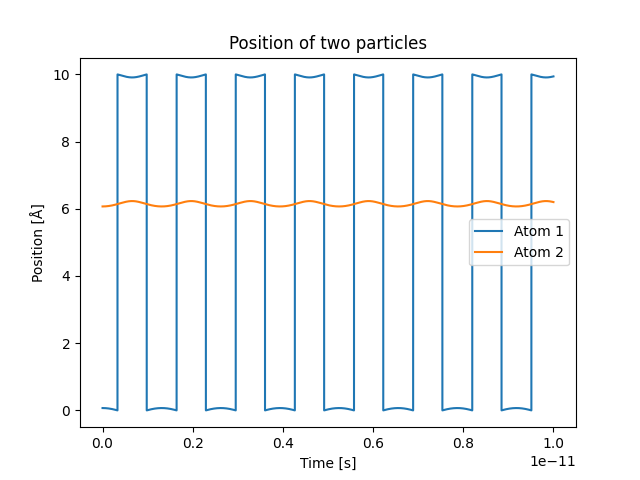
\includegraphics[width=\textwidth]{bsX.png}
        \caption{Position as a function of time $x(t)$ for the two atoms.}
        \label{fig: Position BT}
    \end{subfigure}
    \hfill
    \begin{subfigure}[b]{0.45\textwidth}
        \centering
        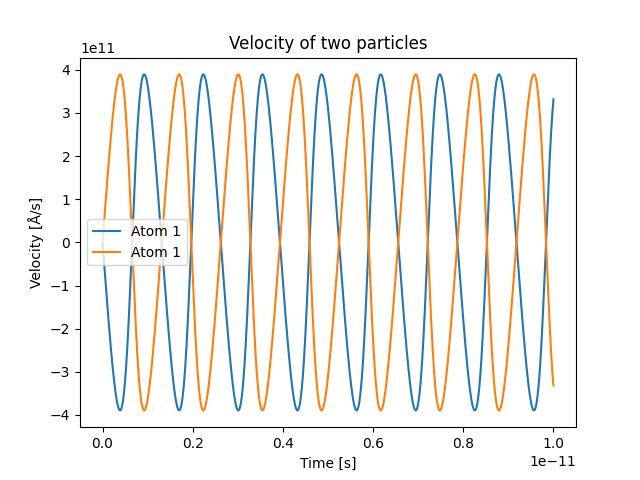
\includegraphics[width=\textwidth]{bsV.png}
        \caption{Velocity as a function of time $v_x(t)$ for the two atoms.}
        \label{fig: Velocity BT}
    \end{subfigure}
    \caption{(a) The atoms position and (b) velocity as a function of time.}
    \label{fig: Position & Velocity Bouncing test}
\end{figure}\noindent
The energy of the system is conserved, as seen by the constant Hamiltonian $\mathcal{H}(t)$ in figure \ref{fig: Energy Bouncing test}.
In the figure it's also shown that the kinetic energy, $\mathcal{K}(t)$ and the potential energy $\mathcal{V}(t)$ oscillates in time.
\begin{figure}[H]
    \centering
    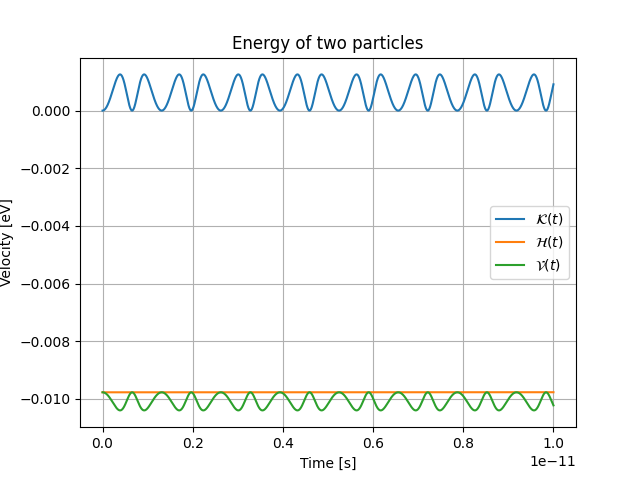
\includegraphics[scale = 0.5]{bsE.png}
    \caption{The energy in the system as a function of time.}
    \label{fig: Energy Bouncing test}
\end{figure}

\subsection{Gas}\label{sec: Gas}
The position of the atoms in the gas are distributed in a uniform manner, as seen in figure \ref{fig: initial position gas}. Here one has $n = 5$ atoms in each dimension, which results in total of $N = 125$ atoms. 
The box-length was determined to be $L = 18.09$~Å, and the density was set to be $\rho = 1.4$~g$/$l.
The atoms are given an initial velocity which is randomized, and the temperature is set to $94.4K$, via the velocity scaling discussed prior, eq \eqref{eq: velocity rescaling}.

\begin{figure}[H]
    \centering
    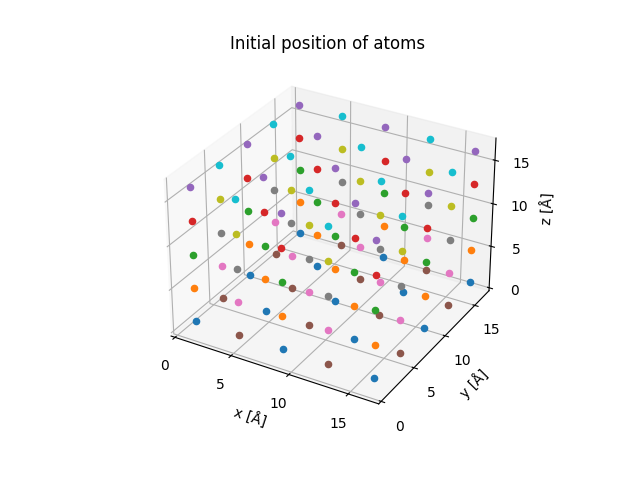
\includegraphics[scale = 0.5]{initial_position.png}
    \caption{The initial position of the atoms in the gas.}
    \label{fig: initial position gas}
\end{figure}\noindent
As seen in the above figure, one has not placed the atoms in a grid spanning the entire volume, but rather in a slightly bulked manner. This is to ensure that the position on the boundaries are not too close to the atoms in the next image, which would result in a stronger interaction between the atoms in the neighboring images.
This would result in a massive force between the atoms, thus also massive accelerations, which now is avoided.
The atoms in the out-most layers, e.g. facing the boundaries, will have stronger interactions with the atoms in the neighboring images, and thus will oscillate in the position, as seen in figure \ref{fig: z-direction-gas}.
\begin{figure}[H]
    \centering
    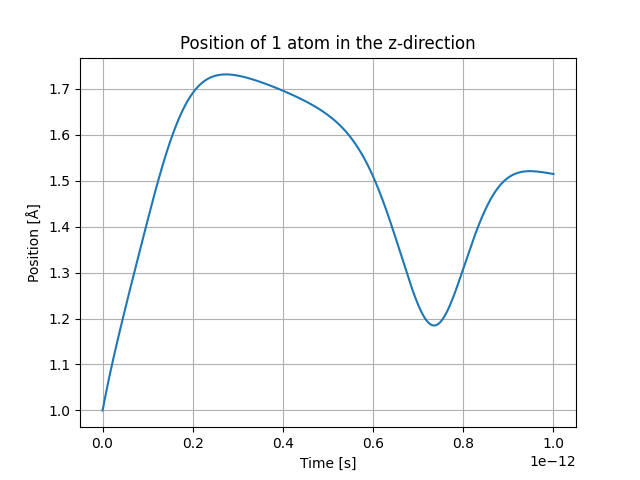
\includegraphics[scale = .5]{pos-z_direction.png}
    \caption{The position of the atom in the $z$-direction as a function of time.}
    \label{fig: z-direction-gas}
\end{figure}\noindent
This behavior is expected throughout the entire bulk, where atoms will vary its position with some small displacement.
The configuration of the atoms, inside the confined volume, is shown in the figure below, where three different instances in time are shown.
\begin{figure}[H]
    \centering
    \begin{subfigure}[b]{0.45\textwidth}
        \centering
        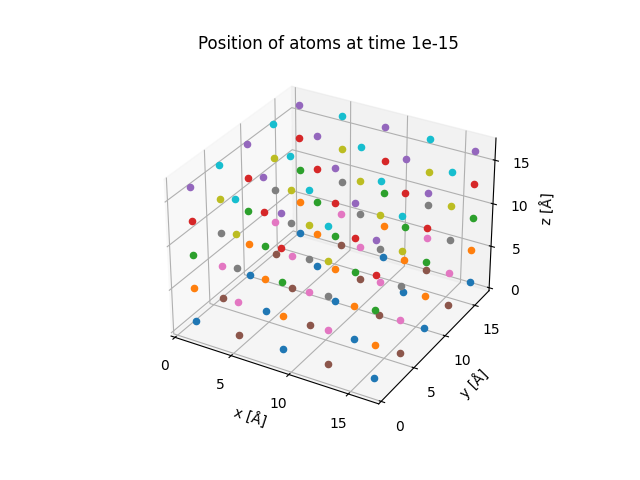
\includegraphics[width=\textwidth]{conf_15.png}
        \caption{Configuration at time $t = 10^{-15}$.}
        \label{fig: Configuration 1}
    \end{subfigure}
    \hfill
    \begin{subfigure}[b]{0.45\textwidth}
        \centering
        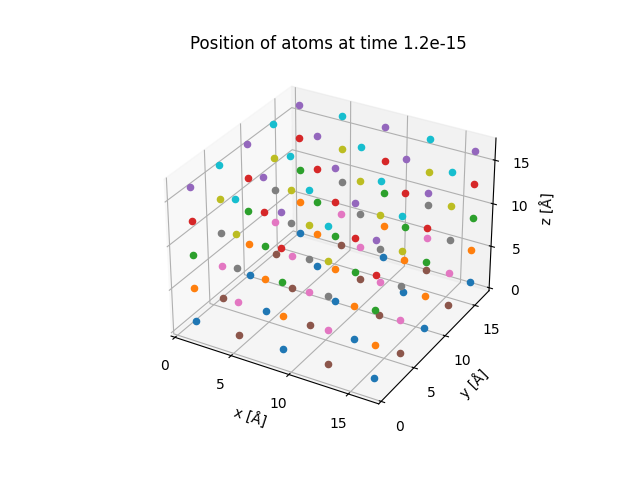
\includegraphics[width=\textwidth]{conf_2_15.png}
        \caption{Configuration at time $t = 2\cdot10^{-15}$.}
        \label{fig: Configuration 2 }
    \end{subfigure}
    \caption{(a) Show the configuration $10\cdot dt$ after the simulation has started. (b) Show the configuration $12\cdot dt$ after the simulation has started.}
    \label{fig: Configuration gas}
\end{figure}\noindent

\begin{figure}[H]
    \centering
    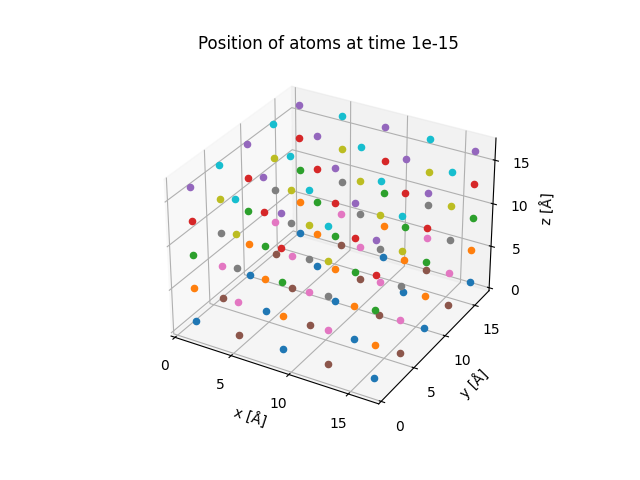
\includegraphics[scale = .5]{conf_15.png}
    \caption{Configuration at time $t = 3\cdot10^{-15}$.}
    \label{fig: Configuration 3}
\end{figure}\noindent
As can be seen in the figure above, there exists no noticeable difference in the configuration of the atoms, within small-time intervals as seen by figure \ref{fig: Configuration 1} and \ref{fig: Configuration 2 }.
The configuration, as time progresses show that the atoms reaches an equilibrium configuration, as seen in figure \ref{fig: Configuration 3}, where they are uniformly distributed in the volume.

\newparagraph
The energies in the system, $\mathcal{V}(t)$, and $\mathcal{K}(t)$ behave different compared to that of the bouncing test, as seen in figure \ref{fig: Energy gas}.
\begin{figure}[H]
    \centering
    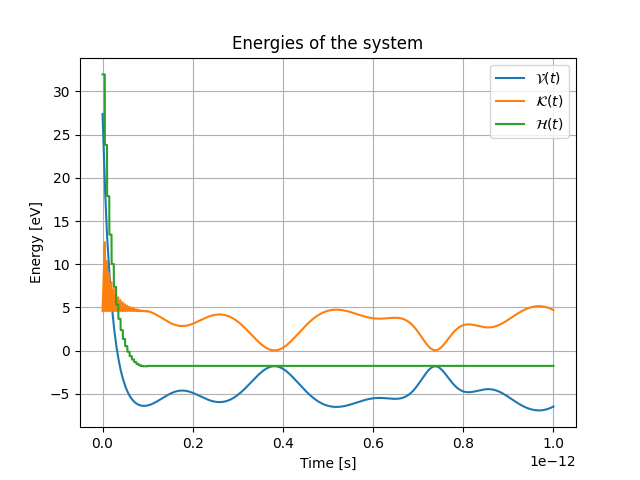
\includegraphics[scale = 0.5]{energy_gas.png}
    \caption{The energy in the system as a function of time.}
    \label{fig: Energy gas}
\end{figure}\noindent
The kinetic energy $\mathcal{K}(t)$ oscillates in time. In the beginning of the simulation, one performs velocity rescaling, eq \eqref{eq: velocity rescaling}, which manifests itself as rapid oscillations, however, as soon as the rescaling ceases the kinetic energy equilibrates.
The potential energy $\mathcal{V}(t)$ also oscillates in time. However, in contrast as to the kinetic energy, the potential is maximized in the beginning of the simulation, and then equilibrates.
The reason for this is due to the large velocities that are induced by the velocity rescaling in the beginning of the simulation, which results in a small relative distance between the atoms, and thus large potential.

\newparagraph
The Hamiltonian $\mathcal{H}(t)$ is not conserved in the beginning of the simulation, however as the velocity rescaling ceases, the Hamiltonian equilibrates, as seen in figure \ref{fig: Energy gas}.
The temperature of the system is shown in the figure below, figure \ref{fig: Temperature gas}.
\begin{figure}[H]
    \centering
    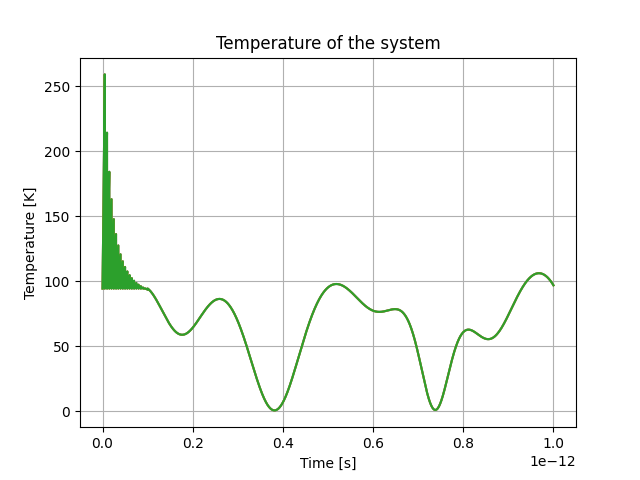
\includegraphics[scale = .5]{temperature.png}
    \caption{The temperature of the system as a function of time.}
    \label{fig: Temperature gas}
\end{figure}\noindent
The temperature of the system, in the beginning of the simulation, is oscillating rapidly due to the velocity rescaling; as time progresses the temperature fluctuations becomes less violent.
The reason for the temperature not being constant can be seen by the direction relationship to the kinetic energy, as seen in eq \eqref{eq: velocity rescaling}. The temperature is proportional to the kinetic energy, and thus the temperature will fluctuate as the kinetic energy fluctuates.
\section{Conclusion}
In this report, one implemented Velocity Verlet method to simulate multiple atoms interacting. The method is fairly efficient, however, in calculating the velocities and such one had to compute the force between the atoms, which is a computationally heavy task.
This task is of time-complexity $\mathcal{O}(N^2)$[2], where $N$ is the number of particles. In the gas simulation, \ref{sec: Gas}, one used $N = 125$ particles.
Therefore, the language of choice, Python, was not suitable for this task, since the language is not optimized for fast computations. In an effort to reduce the computation time, a hash-map was implemented to store already computed forces for all pairs of atoms, and thus, one reduced the computation time.
Hence, in going forward, one should consider writing the code in a more efficient language, such as C++, C or V\footnote{An effort to write the simulation in V was made, however a bug was introduced. Due to lack of time the simulation was never completed in V.}.

\newparagraph
Since the integration method is symplectic, the Hamiltonian should be conserved[3]; this is the case for both the bouncing test and the gas simulation.
This is on par with what was found in the previous report. The temperature fluctuate, as expected, and the kinetic energy and potential energy oscillates in time, which is an expected behavior.

\newparagraph
The integration time in the gas simulation, $T = 1$~ps, is fairly short integration time. One could increase this, to see how the system behaves over a longer period of time, and how the temperature fluctuates over time.
This is something that one should consider in future simulations, where an integration time could extend to $T = 10$~ps instead.
This was not done due to lack of RAM (Random Access Memory) on computer used for the simulations; the method implemented is not optimized for large simulations, and thus the computer ran out of memory when trying to simulate a longer time.

\newpage
\section*{References}
\begin{enumerate}
    \item Bransden, B.H. and Joachain, C.J. (2003) Physics of Atoms and Molecules. Second edition. Pearson Education Limited, 2003. ISBN: 0-582-35492-X.
    \item L. Petterson, (2023, January 27). Lecture 2: Simulation Methods in Statistical Physics, \url{https://athena.itslearning.com/ContentArea/ContentArea.aspx?LocationID=22855&LocationType=1&ElementID=2839898}
    \item L. Petterson, (2024, January 20). Lecture 3: Simulation Methods in Statistical Physics, \url{https://athena.itslearning.com/ContentArea/ContentArea.aspx?LocationID=22855&LocationType=1&ElementID=2839898}
\end{enumerate}





\end{document}
 
